\section{Cipher Specifications}

\begin{frame}{Cipher Specifications}
\begin{block}{}
    \begin{itemize}
    \item Bit-Slice Style
\item Cipher operates over 25 rounds
\item Each round consisting
of three core operations: AddRoundKey (ARK), SubColumn (SC), and ShiftRow (SR)
\end{itemize}
\end{block}

\end{frame}

\begin{frame}{AddRoundkey (AR)}
\begin{block}{}
It is simple XOR operation between the round subkey and the state.
    \begin{figure}[h!]
    \centering
    % First Image
    \begin{subfigure}[b]{1.0\textwidth}
        \centering
        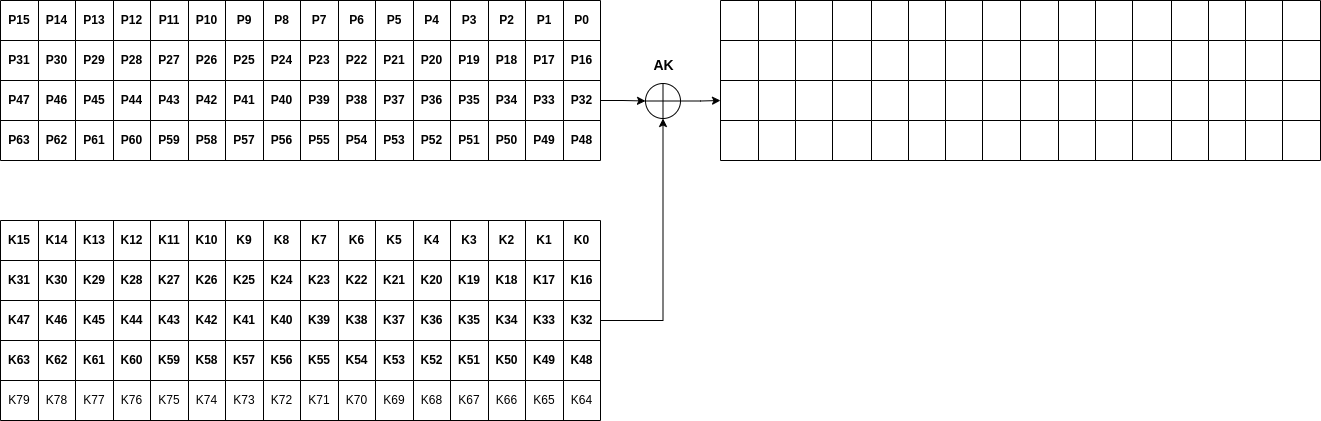
\includegraphics[width=\textwidth]{SKCrypto.drawio.png} 
        \label{fig:image1}
    \end{subfigure}
    \caption{Above diagram shows add round-key operation}
    \label{fig:two_images}
\end{figure}
    
\end{block}
\end{frame}

\begin{frame}{SubColumn (SC)}
\begin{block}{}
SubColumn parallels SubBytes, applying S-boxes to the 4 bits in each column of the state matrix.
\begin{itemize}
    \item Input to the S-box: Col(j) = $a_{3,j} || a_{2,j} || a_{1,j} || a_{0,j}$ for $0 \leq j \leq 15$
    \item Output to the S-box: S(Col(j)) = $b_{3,j} || b_{2,j} || b_{1,j} || b_{0,j}$
\end{itemize}
    \begin{figure}[H]
    \centering
    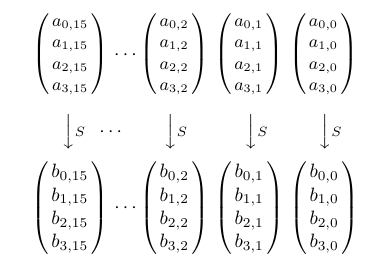
\includegraphics[width=0.4\textwidth]{SubColumn.png}
    \caption*{Figure: Above diagram shows SubColumn operation}
\end{figure}
S-box of Rectangle Cipher-
\begin{figure}
\centering
    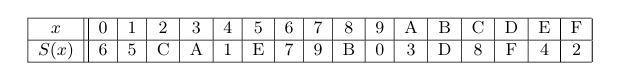
\includegraphics[width=0.8\textwidth]{S-Box.png}
    \caption*{ \textbf{Rectangle Cipher S-Box}}
\end{figure}
    
\end{block}
\end{frame}

\begin{frame}{ShiftRow (SR)}
\begin{block}{}
    It is left rotations on the rows of a state matrix,
with varying offsets for each row.
\begin{figure}[h!]
    \centering
    % First Image
    \begin{subfigure}[b]{1.0\textwidth}
        \centering
        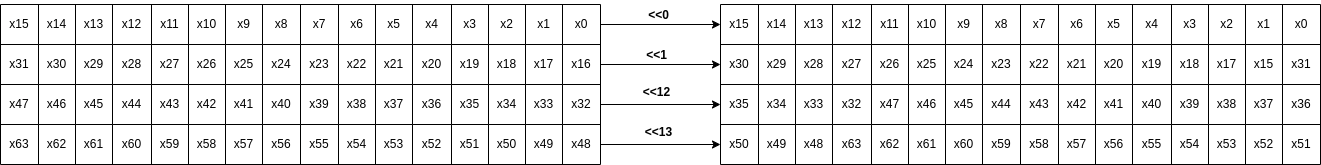
\includegraphics[width=\textwidth]{SR.drawio.png} 
        \label{fig:image1}
    \end{subfigure}
    \caption{Above diagram shows shift row operation}
    \label{fig:two_images}
\end{figure}
    
\end{block}
\end{frame}

\begin{frame}{Pseudo Code}
    \begin{block}{}
    \textbf{GenerateRoundKeys(state)}:\\
\hspace*{1cm}\textbf{for i = 0 to 24 do:}\\
\hspace*{2cm}\textbf{ARK(state,$K_i$)}\\
\hspace*{2cm}\textbf{SC(state)}\\
\hspace*{2cm}\textbf{SR(state)}\\
\hspace*{1cm}\textbf{ARK(state,$K_{25}$)}\\
    \end{block}
\end{frame}

\begin{frame}{Differential Distribution Table (DDT)}
\begin{block}{}
    \begin{figure}[H]
    \centering
    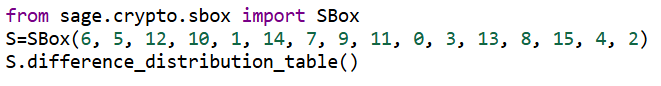
\includegraphics[width=0.7\textwidth]{Screenshot 2024-11-30 141729.png}
    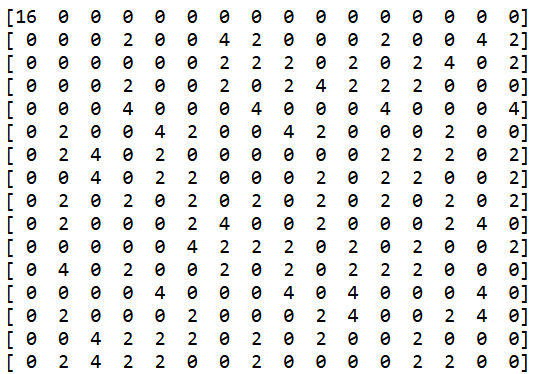
\includegraphics[width=0.7\textwidth]{Screenshot 2024-11-30 141742.png}
\end{figure}
    
\end{block}
\end{frame}

\begin{frame}{Linear Approximation Table (LAT)}
\begin{block}{}
    \begin{figure}[H]
    \centering
    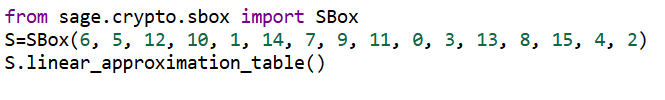
\includegraphics[width=0.7\textwidth]{Screenshot 2024-11-30 142114.png}
    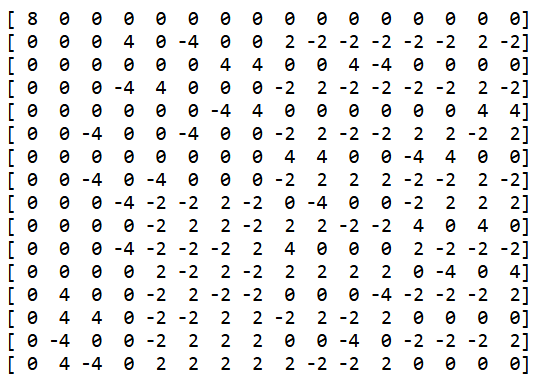
\includegraphics[width=0.7\textwidth]{Screenshot 2024-11-30 142130.png}
\end{figure}
    
\end{block}
\end{frame}

\begin{frame}{Key Schedule}
    \begin{block}{For 80-bit key}
    \begin{enumerate}
        \item SC to the bits at the 4 uppermost rows and the 4 rightmost
columns
\item Using a 1-round generalized Feistel transformation\\
$Row’_0$ := ($Row_0$ << 8) $\oplus$ $Row_1$\\
$Row’_1$ := $Row_2$\\
$Row’_2$ :=$Row_3$\\
$Row’_3$ := ($Row_3$ << 12) $\oplus$ $Row_4$\\
$Row’_4$ := $Row_0$
\item A 5-bit round constant RC[i] is XORed with the 5-bit key
state for i $\in$ (1,2,..,24).
    \end{enumerate}
        
    \end{block}
    
\end{frame}
\begin{frame}{Key Schedule}
    \begin{block}{For  128-bit key}
    \begin{enumerate}
    \item SC to the bits at the 8 rightmost columns.
    \item Using a 1-round generalized Feistel transformation\\
    $Row’_0$ := ($Row_0$ << 8) $\oplus$ $Row_1$\\
    $Row’_1$ := $Row_2$\\
    $Row’_2$ := ($Row_2$ << 16) $\oplus$ $Row_3$ 
    $Row’_3$ := $Row_0$
    \item A 5-bit round constant is XORed with the 5-bit key state
    \end{enumerate}
    \end{block}
\end{frame}
